\documentclass{InsightArticle}

\usepackage[dvips]{graphicx}
\usepackage{float}
\usepackage{subfigure}

\usepackage[dvips,
bookmarks,
bookmarksopen,
backref,
colorlinks,linkcolor={blue},citecolor={blue},urlcolor={blue},
]{hyperref}

\title{Morphological Graph Opening}

% 
% NOTE: This is the last number of the "handle" URL that 
% The Insight Journal assigns to your paper as part of the
% submission process. Please replace the number "1338" with
% the actual handle number that you get assigned.
%
\newcommand{\IJhandlerIDnumber}{3250}

% Increment the release number whenever significant changes are made.
% The author and/or editor can define 'significant' however they like.
\release{0.00}

% At minimum, give your name and an email address.  You can include a
% snail-mail address if you like.

\author{David Doria}
\authoraddress{Army Research Laboratory, Aberdeen MD}


\begin{document}

\IJhandlefooter{\IJhandlerIDnumber}


\ifpdf
\else
   %
   % Commands for including Graphics when using latex
   % 
   \DeclareGraphicsExtensions{.eps,.jpg,.gif,.tiff,.bmp,.png}
   \DeclareGraphicsRule{.jpg}{eps}{.jpg.bb}{`convert #1 eps:-}
   \DeclareGraphicsRule{.gif}{eps}{.gif.bb}{`convert #1 eps:-}
   \DeclareGraphicsRule{.tiff}{eps}{.tiff.bb}{`convert #1 eps:-}
   \DeclareGraphicsRule{.bmp}{eps}{.bmp.bb}{`convert #1 eps:-}
   \DeclareGraphicsRule{.png}{eps}{.png.bb}{`convert #1 eps:-}
\fi


\maketitle


\ifhtml
\chapter*{Front Matter\label{front}}
\fi

\begin{abstract}
\noindent

This document presents an implementation of an algorithm to perform a morphological opening on a graph. The intent is to remove short branches in a graph while preserving the large scale structure.

This implementation is based on the algorithm described in \cite{Sappa}. We have used the data structures from Boost Graph Library (BGL).

The code is available here:
https://github.com/daviddoria/GraphOpening

\end{abstract}

\IJhandlenote{\IJhandlerIDnumber}

\tableofcontents
%%%%%%%%%%%%%%%%%%%%
\section{Introduction}
This document presents an implementation of an algorithm to perform a morphological opening on a graph. This opening consists of a series of erosions, followed by a series of dilations. This is often done as a first step in contour closure algorithms.

This implementation is based on the algorithm described in \cite{Sappa}.

%%%%%%%%%%%%%%%%%%%%
\section{Graph Erosion}
Remove all edges attached to EndPoints (leaf nodes). After multiple iterations of this, small branches
will be "absorbed" into a main branch.

%%%%%%%%%%%%%%%%%%%%
\section{Graph Dilation}
Add back edges to current EndPoints. This is NOT simply going to grow back the same tree. If we ran the erosion enough times
to absorb a branch, the branch will not grow back. If we did not, then the branch will indeed grow back.

%%%%%%%%%%%%%%%%%%%%
\section{Algorithm}
\label{sec:Algorithm}
The algorithm proceeds as follow:
\begin{itemize}
 \item Erode the graph until a stopping criteria is met
 \item Dilate the graph the same number of times as the graph was eroded
\end{itemize}

\subsection{Naive Approach}
At each iteration, erode or dilate the graph while considering nothing about the previous step. In both the erosion and dilation steps, this means finding all of the end points at every iteration, which is the only costly procedure in the algorithm.

\subsection{Speedup}
A list of the remaining vertices after every edge removal is created. These are the only potential candiates which must be determined to be end points or not at the next iteration.

%%%%%%%%%%%%%%%%%%%%
\section{Notes and Behavior}
\begin{itemize}
 \item If an edge was removed in the erosion process, as long as it belonged to the child-most branch that was entirely removed, it will not be regrown in the dilation process.
\end{itemize}


% \begin{figure}[H]
% \centering
% \subfigure[A brown rectangular object.]
%   {
%   
\includegraphics[width=0.3\linewidth]{images/rectangleSolid}
%   \label{fig:EdgeImage:Image}
%   }
% \subfigure[A simple edge pixel classification. White pixels are edge pixels.]
%   {
%   
\includegraphics[width=0.3\linewidth]{images/rectangleSolidEdgeThresholded}
%   \label{fig:EdgeImage:EdgeImage}
%   }
% \caption{An image of an object and its corresponding edge image.}
% \label{fig:EdgeImage}
% \end{figure}

% \begin{figure}[H]
%   \centering
%   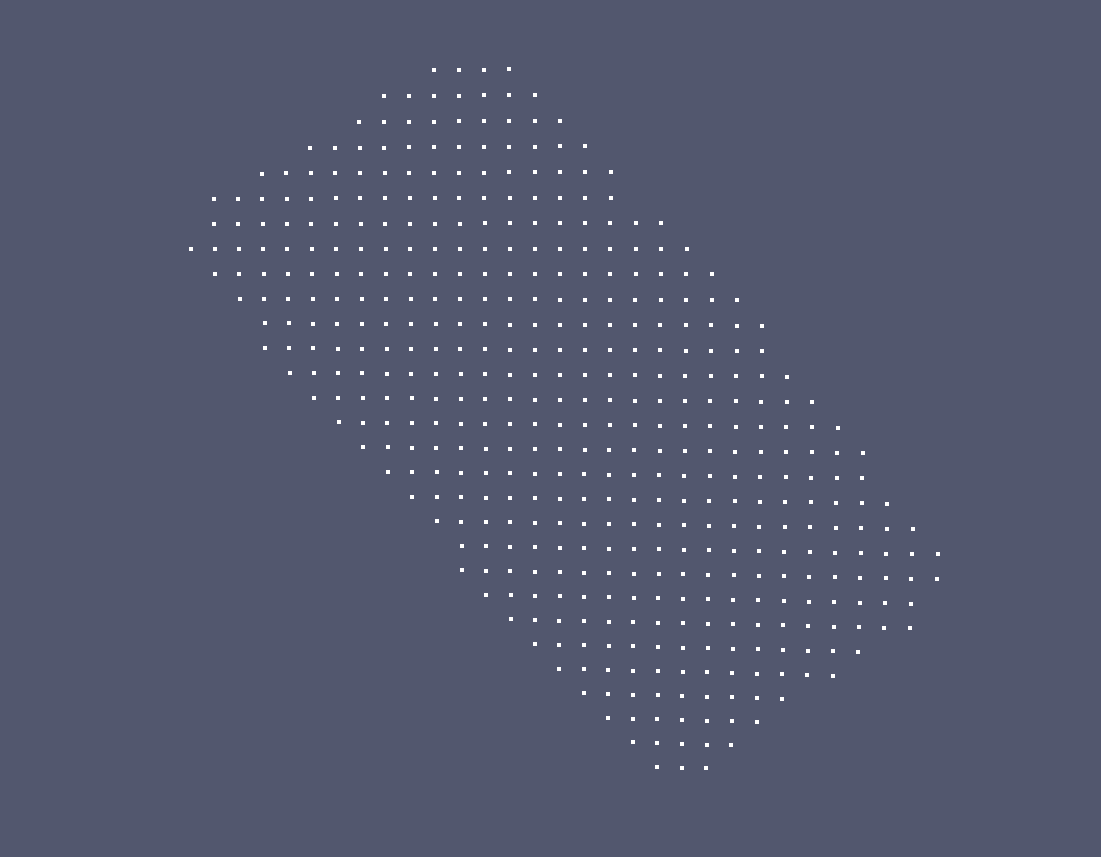
\includegraphics[width=0.3\linewidth]{images/rectanglePoints}
%   \caption{A solid point cloud of a rectangular 2D object.}
%   \label{fig:SolidPointCloud}
% \end{figure}

%%%%%%%%%%%%%%%%%%%%
\section{Demonstration}
\label{sec:Demonstration}

% \begin{figure}[H]
% \centering
% \subfigure[Image to be filled. The region to be filled is shown in bright green.]
%   {
%   \includegraphics[width=0.3\linewidth]{images/BlackWhite}
%   \label{fig:SyntheticDemonstration:ExampleInputImage}
%   }
% \subfigure[The mask of the region to inpaint.]
%   {
%   \includegraphics[width=0.3\linewidth]{images/BlackWhiteMask}
%   \label{fig:SyntheticDemonstration:ExampleInputMask}
%   }
% \subfigure[The result of the inpainting.]
%   {
%   \includegraphics[width=0.3\linewidth]{images/BlackWhiteResult}
%   \label{fig:SyntheticDemonstration:ExampleInputOutput}
%   }
% \caption{Synthetic Demonstration}
% \label{fig:SyntheticDemonstration}
% \end{figure}

%%%%%%%%%%%%%%%
\section{Code Snippet}

\begin{verbatim}

\end{verbatim}


%%%%%%%%%%%%%%%
\begin{thebibliography}{9}

	\bibitem{Sappa}
	  Sappa, A,
	  \emph{Efficient Closed Contour Extraction from Range Image's Edge Points}.
	  Proceedings of the 2005 IEEE International Conference on Robotics and Automation

\end{thebibliography}

\end{document}